\section{Bridging between IB and CB in Java}

\begin{figure}[t]\label{fig:lombok}
\centering
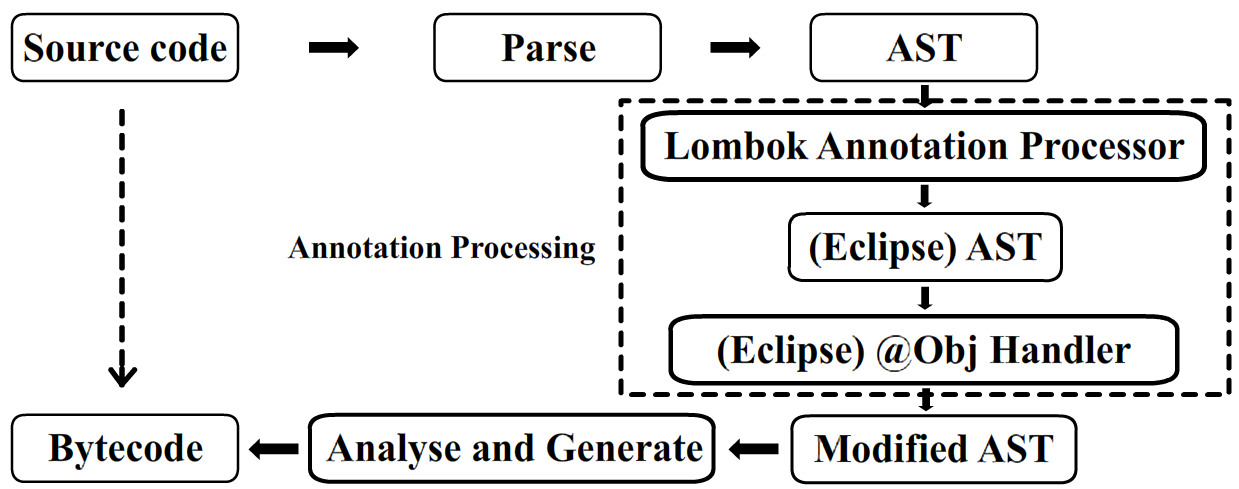
\includegraphics[width=3in]{pdfs/lombok2.png}
\caption{The flow chart of Lombok annotation processing. [Ref: http://notatube.blogspot.hk/2010/12/project-lombok-creating-custom.html]
\marco{I'm not sure this helps: It is trying to show the "eclipse" path, that is the one we implemented,
but there is also the "javac" path, and here we call the graph "Lombok annotation processing".
May be this should be "obj" processing?
}}\bruno{The figure is blurred and the font size is too
small. Hoayuan, please improve the figure.}
\end{figure}


Even if convinced of the advantages of IB, the practical convenience
of using existing libraries points us into building IB support inside
of an opportune CB language like Java.
%\footnote{ Rewriting libraries and
%  application in this language/model would result in more reusable
%  libraries, but it would be a taunting task.}
While creating a new language or language extension would also
illustrate the point of IB (and would be more elegant), it would also
require significant amounts of engineering to achieve a similar level
of integration and tool support as Java.
This section illustrates how we integrate IB directly into Java instead. 
Disciplined use  

\subsection{Compilation Agents}

Java is a good language for such integration, since it supports compilation agents\cite{compilationagents}.
That is, Java libraries can interact with the Java compilation process,
acting as a man in the middle between the
generation of the abstract syntax tree and the Java Bytecode.
\marco{is this correct?}
This process is facilitated by frameworks like Lombock~\cite{lombok}:
a Java library that aims at removing (or
reducing) Java boilerplate code via
annotations.
Figure~\ref{fig:lombok}\haoyuan{Wrong ref?} illustrates the
flow of \mixin annotation processing in Lombok.
%There are a number of annotations provided by the
%original Lombok, including \Q:@Getter:, \Q:@Setter:,
%\Q:@ToString: for generating getters, setters and \QM{toString}
%methods, respectively.  Furthermore, Lombok provides a number of
%interfaces for users to create custom transformations, as extensions
%to the original framework.
%A transformation is based on a handler, which acts on the AST for the
%annotated node and returns a modified AST for analysis and
%generation afterwards. Such a handler can either be a Javac handler or
%an Eclipse handler.

Using Lombok we created our \mixin annotation, that supports object
interfaces as described in the former examples.

Compilation Agents have advantages with respect to
alternatives like extending the language, using a macro pre processors
or using the Java Annotation processors.\marco{are we sure that annotation processors are not compilation agents too?}

Our disciplined \mixin annotation offer some more advantages with respect to arbitrary (Compilation agent driven) AST rewriting.

%this seems like a commercial spot
%\item Lombok is byte-code based instead of source-code based, which makes client
%  code concise and easy to maintain. Such code generation is performed at
%  compile time to modify bytecode.

\paragraph{Auxiliary files/informations do not pollutes the program:}
Compilation Agents alters the generation process of the class files,
by directly modifying the AST.
Neither the source code is modified nor new Java files are generated.
Moreover, and probably more importantly, Lombok supports generation of
  code \emph{inside} a class/interface, which conventional
  Java annotation processors do not support.

\paragraph{Modularity:}
While general preprocessing/macros can act across module boundaries,
Compilation agents act modularly on each class/compilation unit, and it makes
sense to apply the transformation to one class/interface at a time, and only to annotated classes/interfaces.
This allows library code to be reused without the need of being
reprocessed and recompiled, making our approach 100\% compatible with existing Java libraries, than can be used
and extended normally. Of course, Java libraries can also receive and use instances of object interfaces as normal objects.

\paragraph{Tool support:}
Features integrate/supported directly in the language are often also supported by (most) tools.
For example in Eclipse, the processing is performed transparently and the information of
the interface from compilation is captured in the ``Outline'' window. This includes
all the methods inside the interface as well as the generated ones.
This also means that the IDE functionality for content assist and autocomplete
will work for the newly generated methods.


\paragraph{Clarity against Obfuscation:}
Preprocessors bring great power, which can easily be misused producing
code particularly hard to understand. Thus code quality and maintainability are reduced.
Compilation agents start from Java syntax, but they can reinterpret it.
Preserving the syntax avoid syntactic conflicts, and allows may tools to transparently work.

The reinterpretation could still be surprising for badly designed rewritings.
However, ``Outline'' windows/ auto-completion facilities
will show the result of the rewriting, helping the programmer to use the reinterpreted semantic.

Our annotation reinterpret the syntax for the sole goal of enhance/complete code:
we satisfy the behaviour of abstract methods, we add methods and we refine return types.
We consider this to be quite easy to follow, since it is similar to what happens in normal inheritance.

We believe that refactoring operations like rename and move
should work transparently in conjunction with our annotaiton, since they rely on
the overall type structure of the class, that we do not arbitrarily modify but just complete.

%\marco{The section No reuse of the type system
%is controversial.
%We do need to repeat the type checking, plus we aim to make untypable stuff well typed
%(for example anyone using the of method would not be well typed before).}
%\item \textbf{No reuse of the type system.}
%As we mentioned above, badly designed rewritings can arise from the great power of Lombok. A simple piece of source code
%\begin{lstlisting}
%interface M { int m(); }
%\end{lstlisting}
%can be reinterpreted as
%\begin{lstlisting}
%interface M { void m(String s); }
%\end{lstlisting}
%in which case the type of method \Q@m@ is changed. Our \mixin annotation does not introduce this kind of rewritings,
%and hence the type system is reused. Moreover, Lombok can also modify unbounded types, which is easy to understand,
%for instance, the following code
%\begin{lstlisting}
%interface M { T m(); } // T is unbounded
%\end{lstlisting}
%is transformed into
%\begin{lstlisting}
%interface M { int m(); } // No error message
%\end{lstlisting}
%in which case the user will see the unbounded type in source code, but without error message from the compilation, since
%Lombok has modified the return type of \Q@m@. However, our \mixin annotation can still keep such errors and warnings.


%\item \textbf{Lack of reuse.}  %not sure here... I think most preprocessors support decent reuse, even the C one
%Reusability is yet another concern in using preprocessors.
% In Lombok, implementations of features are
%encapsulated in various annotation handlers,
% in which case some behaviours are allowed to reuse the code by invoking methods
%in other handlers, where tedious replicated code is avoided.



\paragraph{Syntax and Type errors:}
Some preprocessors (like the C one) can produce syntactically invalid code.
Lombok ensures only syntactically valid code is produced; however, type errors can appear.

Our annotation is guaranteed to not introduce errors in generate code and client code.
See the following for details, where we identify tree form of types guarantees.


\paragraph{Self coherence}: the generated code itself is well-typed; that is,
  type errors are not present in code the user has not written.
In our case it means that either \mixin{} produces (in a controlled way) an
understandable error, or the interface can be successfully annotated and the generated code is well-typed.
We guarantee \textit{Self coherence}.

\paragraph{Client coherence}: all the client code (for example method calls)
  that is well-typed before code generation is also well-typed after the generation.
The annotation just adds more behaviour without removing any functionality.
We guarantee \textit{Client coherence}.

\paragraph{Heir coherence}: interfaces (and in general classes) inheriting the instrumented code are well-typed if they were well-typed without the instrumentation.
This would forbid adding any (default or abstract) method to the annotated interfaces, including type refinement.
\mixin  does not guarantee \textit{Heir coherence}.
Indeed consider the following:

\begin{lstlisting}
interface A { int x(); A withX(int x); }
@Obj interface B extends A {}
interface C extends B { A withX(int x); }
\end{lstlisting}

\noindent This code is correct before the translation, but \mixin would  generate in \Q@B@  a method ``\Q@B withX(int x);@''.
This would break \Q@C@. \\*
Similarly, an expression of the form ``\Q@new B(){.. A withX(int x){..}}@''
would be correct before translation, but would be ill-typed after the translation.

Our automatic type refinement
is a useful and convenient feature, but not transparent to the heirs of the annotated interface.
They need to be aware of the annotation semantics and provide the right type while refining methods.
Please, note how Java libraries always break heir coherence during evolution
 (is just enough to add any method to any non final class), and still claim backward compatibility
 (false in theory but statistically true in practice).
We think refining return types breaks heir coherence ``less" than normal library evolution.

\paragraph{Type preservation:}
We preferred to introduce self,client and hair coherence instead of referring to conventional
type preservation,
to better model how our approach behave in a object oriented software ecosystem with inheritance,
where only some units may be translated/expanded.
Note inheritance crucial influence in hair coherence, and how client coherence allows
for only some units to be translated/expanded.

This means that even a library designer can decide to start using IB and still
retain backward compatibility with its clients.





\paragraph{Limitations}\marco{ to reorganize with updated limitations}
Our prototype implementation using Lombok has certain limitations:
\begin{itemize}
\item The prototype does not support separate compilation yet. Currently all
  related interfaces have to appear in a single Java file. Therefore, changes to
  a single interface would require re-compiling the whole file. This compilation
  limitation is not caused by our algorithm. It is a Lombok implementation related
  issue: in Lombok it is hard to capture a type declaration from its reference,
  even harder when the type declaration is in other files (we have not found a
  way to do this yet).
\item At this stage our implementation only realizes the Eclipse handler and our
  experiments are all conducted in Eclipse. The implementation for
  \texttt{javac} is missing.
\item The current implementation does not take type-parameters into
  consideration, thus it does not support generics yet.
\end{itemize}

\paragraph{Comparison with other Lombok annotations}\marco{if we keep it, will go in related work}
The Lombok project provides a set of predefined annotations, including constructor
generators similar as ours (e.g., \Q:@NoArgsConstructor:,
\Q:@RequiredArgsConstructor: and \Q:@AllArgsConstructor:). They
generate various kinds of constructors for \emph{classes}, with or without
constructor arguments. This set of annotations is of great use, especially when
used together with other features provided in Lombok (e.g.,
\Q:@Data:). Moreover, the implementation of these annotations in Lombok
gives us hints on how to implement \mixin. However, none of these annotations
can model what we are doing with \mixin - generating constructor-methods
(\textbf{of}) for \emph{interfaces}. Apart from constructors, \mixin also
provides other convenient features (including generating fluent setters, type
refinement, etc), which the base Lombok project does not provide.
Finally, while \mixin is formalized, none of Lombok's annotations have been
studied in a formal way.

%\paragraph{Lombok does language tuning}
%We consider Lombok to be the most developed example of language
%tuning.  While the authors of Lombok do not introduce a specific term
%for what they are doing, their slogan \emph{``Spice up your java''}
%seems to be in line with the philosophy of language tuning. Some
%other examples of language tuning in Lombok include the \Q@val@ type,
%similar to \Q@auto@ in C\# or C++04.  Another library doing language
%tuning is CoFoJa~\cite{cofoja}, where annotations are used to insert
%pre-post conditions in generated bytecode.

